\chapter{振动和波}

\section*{A 组}
\vspace{0.3cm}
\textbf{7-1} 一质点沿 $x$ 轴作简谐振动, 其运动方程为
\[
x = 0. 4 \cos 3 \pi \left(t + \frac {1}{6}\right),
\]
式中 $x$ 和 $t$ 的单位分别是 $m$ 和 $s$. 试求：

(1) 振幅、角频率和周期；

(2) 初相位、初位置和初速度；

(3) t=1.5s 时的位置、速度和加速度.

\vfill

\textbf{7-2} 一简谐振动的运动方程为

\[
x = 5 \cos \left(8 t + \frac {\pi}{4}\right),
\]
为使其初相位为零,计时零点应提前或推迟若干?

\vfill

\newpage

\textbf{7-3} 简谐振动的正弦表达式为 $x = A \sin(\omega t + \phi)$ ，仍称 $\omega t + \phi$ 为其 $t$ 时刻的相位.一质点作正弦简谐运动, 在某一相位时, 它的位置是 $x_0 > 0$ , 当相位增大一倍时, 它的位置是 $\sqrt{3} x_0$ , 试求振幅 $A$ .

\vfill

\textbf{7-4} 设同时有以下三个简谐振动：
\[
x _ {1} = A \sin \omega t,x _ {2} = A \sin \left(\omega t + \frac {2}{3} \pi\right),x _ {3} = A \sin \left(\omega t - \frac {2}{3} \pi\right).
\]

(1) 写出 $x_{2}, x_{3}$ 对 $x_{1}$ 的相位差；

(2) 将这三个振动改用余弦函数表述, 且规定初相位的绝对值不可超过 $\pi$ , 再写出 $x_{2}, x_{3}$ 对 $x_{1}$ 的相位差.

\vfill

\newpage

\textbf{7-5} 一简谐振动为 $x = 2\cos (\pi t + \phi)$ ，试画出 $\phi = 0$ 或 $\phi = \pi /3$ 对应的 $x - t$ 曲线.

\vfill

\textbf{7-6} 求以下两组一维振动的合振动：

(1) $x_{1} = 8\cos \left(\omega t + \frac{3}{8}\pi\right), x_{2} = 6\cos \left(\omega t - \frac{1}{8}\pi\right)$ ;

(2) $x_{1} = A\cos \omega t, x_{2} = A\cos \left(\omega t + \frac{2}{3}\pi\right), x_{3} = A\cos \left(\omega t - \frac{2}{3}\pi\right)$ .

\vfill

\newpage

\textbf{7-7} 已知两个分振动 $x_{1} = 3A\cos \omega_{0}t, x_{2} = A\cos 3\omega_{0}t$ ，试画出 $x_{1} - t, x_{2} - t$ 曲线和合振动 $x = x_{1} + x_{2}$ 随 $t$ 变化的曲线，据此判定合振动是周期振动.

\vfill

\textbf{7-8} 某振动量 $x$ 随时间 $t$ 的变化关系为
\[
x = A _ {0} (1 + \alpha \cos \Omega t) \cos \omega t,
\]
式中 $A_0, \alpha, \Omega, \omega$ 都是正的常量，且 $\alpha < 1, \Omega \ll \omega$ .

(1) 简述 x-t 振动中包含的拍现象, 并写出拍频 $\nu_{拍}$ ;

(2) 将 x-t 振动分解为若干个简谐振动.

\vfill

\newpage

\textbf{7-9} 质点同时参与的两个垂直方向简谐振动分别为

(1) $x = A\cos \omega t, y = B\sin \omega t;$

(2) $x = A\sin \omega t, y = B\cos \omega t.$

试画出质点的两种运动轨道,并标明质点运动方向.

\vfill

\textbf{7-10} 在倾角为 $\theta$ 的光滑斜面上放置一个质量为 $m$ 的小物块, 小物块与一轻弹簧相连, 弹簧的另一端固定在斜面上, 弹簧的劲度系数为 $k$ , 以小物块平衡位置为原点, 沿斜面设置向下的 $x$ 轴. 将小物块从其平衡位置向下拉到 $l$ 距离处, 如图所示, 当 t=0 时刻静止地释放小物块. 试求小物块的振动周期并写出小物块振动表达式 x-t.

\begin{center}
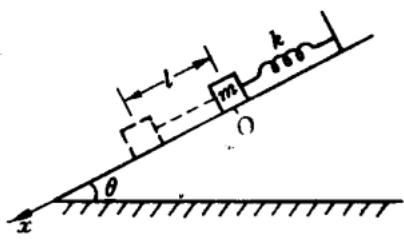
\includegraphics[width=0.3\textwidth]{figures/图7_7.jpg}
\end{center}

\vfill

\newpage

\textbf{7-11} 系统如图所示, 质量 $m$ 的小物块与水平地面光滑接触,劲度系数分别为 $k_{1}, k_{2}$ 的两个轻弹簧开始时均处于自由长度状态. 若使小物块获得朝右(或朝左)的初速度,便会形成振动,试求振动周期 $T$.

\begin{center}
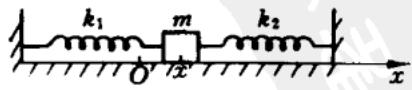
\includegraphics[width=0.3\textwidth]{figures/图7_8.jpg}
\end{center}

\vfill

\textbf{7-12} 系统如图所示, 动滑轮、细绳及两弹簧的质量均可忽略, 细绳与滑轮间无摩擦, 有关参量已在图中示出. 让悬挂物在竖直方向上偏离平衡位置, 便可形成简谐振动, 试求振动周期 $T$. 如果要求悬挂物的运动是纯粹的简谐振动 (即在简谐振动过程中始终不会有其他形式的运动), 振幅 $A$ 将有何限制?

\begin{center}
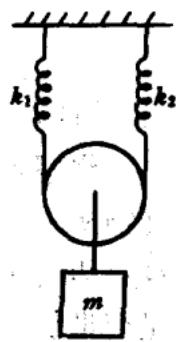
\includegraphics[width=0.1\textwidth]{figures/图7_9.jpg}
\end{center}

\vfill

\newpage

\textbf{7-13} 如图所示, 由劲度系数为 $k$ 的轻弹簧和质量为 $M$ 的振子组成的水平简谐振动系统, 其振幅为 $A$. 一块质量为 $m$ 的黏土从静止状态粘到振子上, 试问在以下两种情形下，振动周期和振幅的变化：

(1) 当振子通过其平衡位置时与黏土相粘；

(2) 当振子在最大位移处与黏土相粘.

\begin{center}
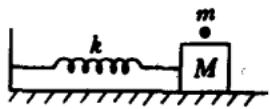
\includegraphics[width=0.3\textwidth]{figures/图7_10.jpg}
\end{center}

\vfill

\textbf{7-14} 系统如图所示, 弹簧及细绳质量均可忽略, 滑轮不能转动, 滑轮与细绳之间无摩擦, 已知量均已在图中示出. 不考虑绳弯折的可能性, 试求滑轮的上下振动周期 $T$.

\begin{center}
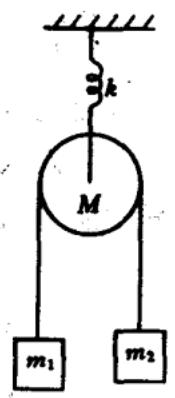
\includegraphics[width=0.1\textwidth]{figures/图7_11.jpg}
\end{center}

\vfill

\newpage

\textbf{7-15} 匀质柱形木块浮在水面上, 水中部分深度为 $h$ , 如图所示. 今使木块沿竖直方向振动, 过程中顶部不会浸入水中, 底部不会浮出水面, 不计水的运动, 略去木块振动过程中所受阻力, 试求振动周期 $T$ .

\begin{center}
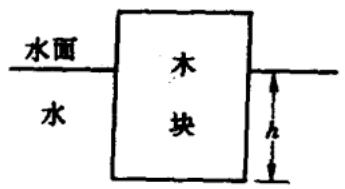
\includegraphics[width=0.3\textwidth]{figures/图7_13.jpg}
\end{center}

\vfill

\textbf{7-16} 两位外星人 $A$ 和 $B$ 生活在一个没有自转、没有大气、表面光滑的匀质球形小星球上。有一次他们决定进行一次比赛，从他们所在的位置出发，各自采用航天技术看谁能先到达星球的对径位置。 $A$ 计划穿过星体直径凿一条通道，采用自由下落方式到达目标位置； $B$ 计划沿着紧贴星球表面的空间轨道，像人造卫星一样航行到目标位置。试问 $A$ 与 $B$ 谁会赢得这场比赛？

\vfill

\newpage

\textbf{7-17} 由一长为 $l$ 、质量为 $m$ 的匀质杆和一质量为 $m_0$ 、半径为 $R$的匀质圆盘,通过盘心固连方式组成的复摆如图所示,试求小角度摆动周期$T$和等时摆长$L$.

\begin{center}
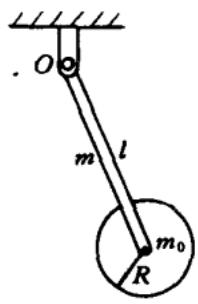
\includegraphics[width=0.2\textwidth]{figures/图7_15.jpg}
\end{center}

\vfill

\textbf{7-18} 竖直平面内有一半径为 $R$ 的光滑固定圆环, 长 $R$ 的匀质细杆放在环内, 试求杆在其平衡位置两侧小角度摆动周期 $T$.

\begin{center}
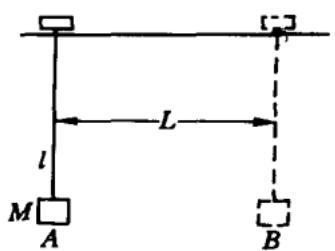
\includegraphics[width=0.3\textwidth]{figures/图_7_17.jpg}
\end{center}

\vfill

\newpage

\textbf{7-19} 如图所示, 吊车拟用长 $l$ 、质量可忽略的绳索将重物 $M$ 从 $A$ 移动到 $B$ , 其间水平距离为 $L$ . 设吊车以匀加速度 $a$ 从静止出发经 $L/2$ 路程后, 又以反向加速度 $a$ 减速经过余下的 $L/2$ 路程. 要求重物在 $A, B$ 位置均处于静止状态, 且在运动过程中作小角度摆动, 略去小重物的线度, 试求可取的 $a$ 值. (小角度单摆的幅角约束在 $5^\circ$ 范围之内.)


\vfill

\textbf{7-20} 如图所示, 质量 $m = 121 \mathrm{~g}$ 的水银盛在截面积 $S = 0.30 \mathrm{~cm}^{2}$ 的竖直开口 $U$ 形管内, 从试管一端朝里轻轻吹一口气, 管内水银面便会上下振动. 已知水银密度 $\rho = 13.6 \mathrm{~g} / \mathrm{cm}^{3}$ , 略去水银与管壁间的黏力, 试求水银面振动周期 $T$ .

\begin{center}
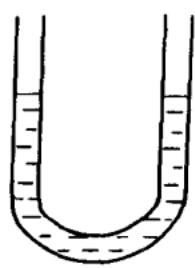
\includegraphics[width=0.1\textwidth]{figures/图_7_18.jpg}
\end{center}

\vfill

\newpage

\textbf{7-21} 系统如图所示, 平衡时两个水平轻弹簧都处于自由长度状态, 平板左右振动时, 下面两个相同的匀质圆柱体沿水平地面纯滚动, 与平板下表面间也无相对滑动. 已知两个弹簧的劲度系数同为 $k$, 平板质量为 $M$, 两个圆柱体的质量同为 $m$, 试求平板左右振动的周期 $T$.

\begin{center}
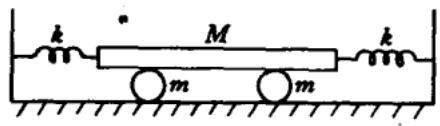
\includegraphics[width=0.3\textwidth]{figures/图7_19.jpg}
\end{center}

\vfill

\textbf{7-22} 系统如图所示, 轻绳与实心匀质滑轮之间无相对滑动,试用能量方法求解滑轮右侧悬挂物在其平衡位置附近的简谐振动周期 $T$. 若要求悬挂物作纯粹的简谐振动(即其间无其他形式的运动参与),那么对振幅 $A$ 的取值有何要求?

\begin{center}
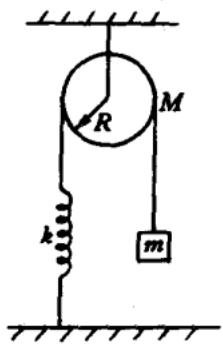
\includegraphics[width=0.2\textwidth]{figures/图7_20.jpg}
\end{center}

\vfill

\newpage

\textbf{7-23} 质量 $M$、半径 $R$ 匀质圆盘，在光滑水平面上可绕过中心$O$ 的固定竖直轴无摩擦地自由转动. 两根自由长度同为 $\pi R/2$ 、劲度系数同为 $k$ 的轻弹簧, 各自一端固连在圆盘直径 AB 的两个端点, 另一端共同连接质量为 $m$ 的小球 $P$, 弹簧与小球可沿着圆盘外侧壁无摩擦地运动. 开始时系统处于静止状态, $P$ 与 $A$ 点之间的圆弧 AP 相对圆心 $O$ 所张圆心角为 $60^{\circ}$ , 如图所示. 将系统自由释放后, 便会往返运动, 设定 $M = 2m$ , 试求:

(1) 运动过程中 $P$ 的最大速度 $v_{max}$ ;

(2) 系统运动周期 $T$.

\begin{center}
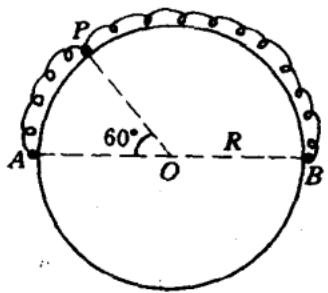
\includegraphics[width=0.2\textwidth]{figures/图7_21.jpg}
\end{center}

\vfill

\textbf{7-24} 质量为 $M$ 的电梯用钢丝绳索吊住, 绳索质量不计, 绳索中的张力 $T$ 与绳索伸长量 $\Delta l$ 之间的关系是 $T = \alpha (\Delta l)^{2}$ , 其中 $\alpha$ 为正的常量. 试求电梯在其平衡位置上下作竖直方向微小振动的周期 $T$ .

\vfill

\newpage

\textbf{7-25} 冰的密度记为 $\rho_{1}$ ，海水速度记为 $\rho_{2}$ ，有 $\rho_{1}<\rho_{2}$ 。金字塔形（正四棱锥形）的冰山漂浮在海水中，平衡时塔顶离水面高度为 $h$，试求冰山在平衡位置附近作竖直方向小振动的周期 $T$。

\vfill

\textbf{7-26} 试由 t=0 时振子的位置 $x_{0}$ 和速度 $v_{0}$ ，确定临界阻尼振动 $x=(A_{1}+A_{2}t)\mathrm{e}^{-\beta t}$ 中的待定常量 $A_{1}$ 和 $A_{2}$ .


\vfill

\newpage

\textbf{7-27} 质量 $m_{1}=10\ kg$ 的物体从 $h=0.50\ m$ 高处静止下落到弹簧秤的秤盘里，并粘附在盘上。已知秤盘质量 $m_{2}=2.0\ kg$ ，弹簧的劲度系数 $k=980\ kg/s^{2}$ ，为使秤盘在最短时间内停下，就须附上一个阻尼系统，试求所需的阻尼系数 $\beta$ 。将振子的力平衡点取为坐标原点，设置竖直朝下的 $y$ 轴，再将物体落到秤盘瞬间取为 t=0 时刻，试写出 $t\geqslant0$ 时振子的运动方程 y-t。

\vfill

\textbf{7-28} 阻尼振动中振子的固有角频率 $\omega_0$ 恰是阻尼系数 $\beta$ 的 $\sqrt{2}$ 倍，已知 $t = 0$ 时振子位于 $x_0 > \zeta$ 处，振动速度 $v_0 = -2\beta x_0$ ，试求振子的运动方程 $x \sim t$ .

\vfill

\newpage

\textbf{7-29} 摆长 l=0.750m 的单摆作阻尼振动，经 $\Delta t=1\min$ 后，其振幅减为初始振幅的 1/8，试求对数减缩 $\lambda$ .

\vfill

\textbf{7-30} 在某钢琴上弹响中音 $C$ 这个琴键时, 其振动能量在 $\Delta t = 1 \, s$ 内减至初始值的一半. 已知中音 $C$ 的频率 $f_{0} = 256 \, Hz$ , 试求系统品质因数 $Q$.

\vfill

\newpage

\textbf{7-31} 固有角频率为 $\omega_{0}$ 的振子，在作受迫振动达到稳定态时，振动速度恰好与驱动力同相位，试求驱动力角频率 $\omega$ .

\vfill

\textbf{7-32} 固有频率为 2.0 Hz 的弹簧振子, 所受空气阻力的大小与振子速度成正比. 对振子施以振幅为 $1.0 \times 10^{-3}$ $N$ 的谐变力, 发生振幅为 5.0 cm 的共振. 设空气阻力系数 $\gamma$ 是个小量, 试求 $\gamma$ 和阻力的幅度(即阻力的最大值) $f_{M}$ .

\vfill

\newpage

\textbf{7-33} 设受迫振动中的驱动力为 $F = F_{0} \cos^{2} \omega t$ ，即振子的动力学微分方程可表述为
\[
\ddot {x} + 2 \beta \dot {x} + \omega_ {0} ^ {2} x = f _ {0} \cos^ {2} \omega t,
\]
试以 $\beta, \omega_0, f_0$ 和 $\omega$ 为已知参量，给出振子的稳态解.

\vfill

\textbf{7-34} 人耳能听到的声音, 其频率范围在 20\textasciitilde{}20000 Hz 间. 已知声波在 25 ℃ 海水中的传播速度为 1531 m/s, 试计算人耳在 25 ℃ 海水中能听到的声音的波长范围.


\vfill

\newpage

\textbf{7-35} 人眼所能见到的光的波长范围是 $400 \sim 760 \mathrm{~nm}$ , 求可见光的频率范围. 人眼最敏感的光是黄绿色光, 波长为 $550 \mathrm{~nm}$ , 求黄绿光波的频率.


\vfill

\textbf{7-36} 设有一列简谐横波：
\[
y = 5. 0 \cos 2 \pi \left(\frac {t}{0 . 0 5} - \frac {x}{1 0}\right),
\]
其中 $x, y$ 的单位是 $\mathrm{cm}, t$ 的单位是 $\mathbf{s}$ . 试求:

(1) 振幅 $A$, 角频率 $\omega$ , 波速 $u$ 和波长 $\lambda$ ;

(2) 振动初相位是 $\frac{3}{5}\pi$ 的位置 $x$ .


\vfill

\newpage

\textbf{7-37} 一列简谐横波沿某弦线自左向右传播,传播速度为80cm/s.观察弦上某点的运动,发现该点在作振幅为2cm,频率为10Hz的简谐振动.取该点为坐标原点,设置自左向右的$x$坐标,已知t=0时该点振动量y=0,且振动速度沿$y$轴正方向.试求:

(1) 此波的波长 $\lambda$ ;

(2) 弦上该点振动的运动学方程；

(3) 弦波的运动学方程；

(4) 弦上 $x=4\,cm$ 处质点振动的初相位 $\phi_{x}$ .

\vfill

\textbf{7-38} 某平面简谐波在 t=0 时刻的波形曲线如图所示, 波朝 $x$ 轴负方向传播, 波速 u=330 m/s, 试写出波函数 $\xi(x,t)$ 表达式.

\begin{center}
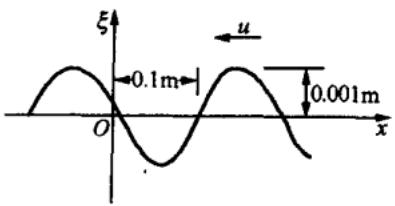
\includegraphics[width=0.3\textwidth]{figures/图7_22.jpg}
\end{center}

\vfill

\newpage

\textbf{7-39} 在介质中传播速度 $u=200\ cm/s$ ，波长 $\lambda=100\ cm$ 的一列平面简谐波, 某时刻的一部分波形曲线如图所示. 已知图中 $A$ 点坐标 $x_{A}=20\,cm$ , 振动量 $\xi_{A}=4\,cm$ , 振动速度 $v_{A}=12\pi\,cm/s$ , 以此时刻开始计时, 写出 $x_{B}=95\,cm$ 处 $B$ 点的振动表述式.

\begin{center}
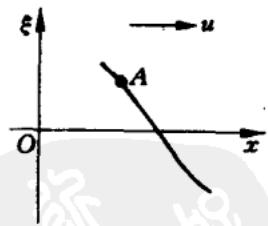
\includegraphics[width=0.3\textwidth]{figures/图_7_23.jpg}
\end{center}

\vfill

\textbf{7-40} 波长为 $\lambda$ 的平面简谐波在 x=0 处的振动曲线如图所示，其中 $\omega$ 为振动角频率。试在 $\xi-x$ 坐标平面上画出 t=0 与 t=T/4 时刻的波形曲线，此处 $T$ 为振动周期。

\begin{center}
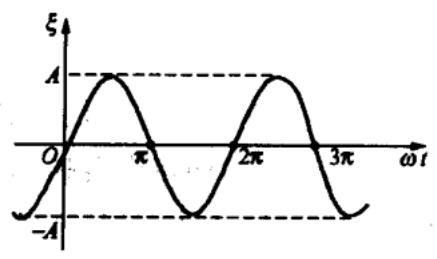
\includegraphics[width=0.3\textwidth]{figures/图7_24.jpg}
\end{center}

\vfill

\newpage

\textbf{7-41} 为测定声音振动频率,采用干涉法,如图所示. 图中 $T$ 是声源, $A$, $B$ 是两根弯头,均为空的金属管,弯管 $B$ 可以移动,$C$ 处 $M$ 是助听器. 观察者移动弯头 $B$ 的位置,用助听器来监听调节声音的增强或减弱. 为使声音强度从一个极小值过渡到下一个极小值,将弯管 $B$ 移动距离 $l=5.5 cm$. 在室温下声波速度 $u=340 m/s$,试求声音振动频率 ν.

\vfill

\textbf{7-42} 如图所示, 拉直的绳子左端固定于墙上, 简谐绳波自 $x$ 轴正方向的远处沿 $x$ 轴负方向入射而来, 入射波在坐标原点 $O$ 的振动为 $\xi_{0}=A\cos\omega t$ , $O$ 点与墙的距离为 $\frac{5}{4}\lambda$ , 其中 $\lambda$ 为入射波长.

入射波遇绳固定于墙的端点将发生反射, 反射波的振幅仍为 $A$, 角频率仍为 $\omega$ , 波长仍为 $\lambda$ , 但相位有 $\pi$ 突变, 使绳的固定端合振动为零. 反射波与入射波在绳中将叠加成驻波, 试导出驻波方程, 并画出驻波的波形曲线.

\begin{center}
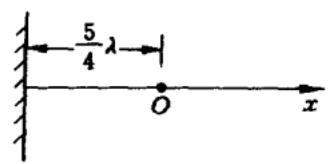
\includegraphics[width=0.3\textwidth]{figures/图7_28.jpg}
\end{center}

\vfill

\newpage

\textbf{7-43} 如图所示, 在竖直峭壁左侧地面上有一辆警车 $S$ 以$v_{S}=10\ m/s$ 的速度朝着峭壁开去, 同时发出频率 $\nu_{0}=1000\ Hz$ 的警笛声. 在警车左侧有一骑自行车者 $B$, 他以 $v_{B}=2\ m/s$ 的速度背向峭壁离去. 设声波在空气中的传播速度 $u=330\ m/s$ , 试求 $B$ 接收到的两种声波频率.

\begin{center}
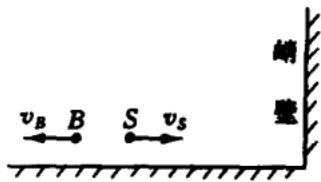
\includegraphics[width=0.3\textwidth]{figures/图_7_30.jpg}
\end{center}

\vfill

\textbf{7-44} 一人手执一音叉向一高墙以 5 m/s 的速度跑去, 音叉的频率为 500 Hz, 声波传播速度为 330 m/s, 试计算此人所听到的声音的拍频.


\vfill

\newpage

\textbf{7-45} 放置在海底的超声波探测器发出一束频率为 30000 Hz 的超声波, 被迎面驶来的潜水艇反射回探测器来, 测得反射波频率与原发射频率差为 241 Hz. 已知超声波在海水中的传播速度为 1500 m/s, 试求潜水艇航行速度 $v$.


\vfill

\textbf{7-46} 如图所示, 一根线密度 $\lambda_{m}=0.15\ g/cm$ 的弦线, 其一端与频率 $\nu=50\ Hz$ 的音叉相连，另一端跨过定滑轮后悬一重物给弦线提供张力，音叉到滑轮间的距离 l=1 $m$. 当音叉振动时，设重物不振动，为使弦上形成有一个、二个、三个波腹的驻波,则重物的质量 $m$ 应各为多大?

\begin{center}
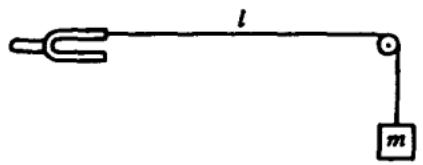
\includegraphics[width=0.3\textwidth]{figures/图7_31.jpg}
\end{center}

\vfill

\newpage

\textbf{7-47} 已知弦线质量线密度为 $\lambda$ ，弦中张力为 $T$ ，弦中简谐横波的运动方程为 $\xi = A\left[\omega\left(t - \frac{x}{u}\right) + \phi\right]$ ，试求弦波的能量线密度（单位长度上波的能量） $\epsilon$ 。

\vfill

\section*{B 组}
\vspace{0.3cm}
\textbf{7-48} 两个同方向、不同频率的简谐振动,如果初相位相同,振幅不同,则可分别记为
\[
x _ {1} = A _ {1} \cos \omega_ {1} t, \quad x _ {2} = A _ {2} \cos \omega_ {2} t.
\]
利用三角函数和差化积公式,这两个简谐振动的合振动可表述成
\[
\begin{array}{l} x = x _ {1} + x _ {2} = \frac {1}{2} (A _ {1} + A _ {2}) (\cos \omega_ {1} t + \cos \omega_ {2} t) \\ + \frac {1}{2} (A _ {1} - A _ {2}) (\cos \omega_ {1} t - \cos \omega_ {2} t) \\ = \left(A _ {1} + A _ {2}\right) \cos \left(\frac {\omega_ {1} - \omega_ {2}}{2} t\right) \cos \left(\frac {\omega_ {1} + \omega_ {2}}{2} t\right) \\ + \left(A _ {2} - A _ {1}\right) \sin \left(\frac {\omega_ {1} - \omega_ {2}}{2} t\right) \sin \left(\frac {\omega_ {1} + \omega_ {2}}{2} t\right), \\ \end{array}
\]
即可分解成两个拍的叠加. 为方便称第一项为“大拍”, 称第二项为“小拍”.

由太阳引起的太阳潮和由月球引起的月亮潮，均可近似处理为简谐振动。太阳潮的振幅为0.5m，周期为12h（小时）；月亮潮的振幅为0.8m，周期为12.5h。太阳潮与月亮潮合成的海水潮汐（海面振动）也可分解成两个拍的叠加，“大拍”达最大幅度 $A_{大}$ 时对应的潮汐称为大潮，“小拍”达最大幅度 $A_{小}$ 时对应的潮汐称为小潮。设海水足够深，试求 $A_{大}, A_{小}$ 和相邻大潮与小潮之间的时间间隔 $\Delta t$ 。


\vfill

\newpage

\textbf{7-49} 在一劲度系数为 $k$ 的竖直轻长弹簧下端连接着质量为 $m$ 的小球, 开始时小球静止地处于力平衡态. 设 $t = 0$ 时刻开始, 弹簧上端以匀速度 $u$ 竖直向上运动, 到 $t = t_0$ 时刻又突然降速到零. 建立附着于弹簧上端且竖直向下的 $x$ 坐标轴, 其原点选在 $t = 0$ 时刻小球所处位置, 试在 $t \geqslant 0$ 的范围确定小球位置 $x$ 随时间 $t$ 变化的函数关系.

\vfill

\textbf{7-50} 图 7-32 所示的水平弹簧振子中, 劲度系数为 $k$ 的轻弹簧自由长度足够长. 将质量为 $m$ 的振子水平向右移动, 直到弹簧伸长 $L$ , 而后将振子自由释放. 已知振子与水平地面间的摩擦因数为常量 $\mu$ , 试问若振子运动过程中至少停止过两次, 那么第二次停留的位置相对振子的初始位置在何处?

\begin{center}
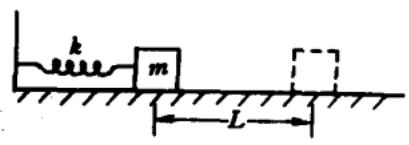
\includegraphics[width=0.3\textwidth]{figures/图7_32.jpg}
\end{center}

\vfill

\newpage

\textbf{7-51} 如图所示, 在水平地面上方高 1 $m$ 处有一固定的水平横杆, 横杆下用细线悬挂着小球 $A$, $A$ 通过一根轻弹簧与另一个相同的小球 $B$ 相连. $A$, $B$ 静止不动时, 弹簧伸长 3.0 cm. 今将细线烧断, $A$, $B$ 便与弹簧一起下落, 假设 $B$ 触及地面上的橡皮泥时, 弹簧的伸长量正好也是 3.0 cm, 而后 $B$ 与橡皮泥发生完全非弹性碰撞. 考虑到 $A$ 将会继续朝下运动, 试求而后弹簧相对其自由长度的最大压缩量.

\begin{center}
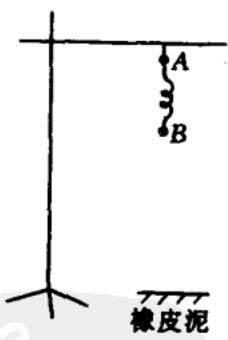
\includegraphics[width=0.15\textwidth]{figures/图7_34.jpg}
\end{center}

\vfill

\textbf{7-52} 在光滑的水平桌面上开有一小孔, 一根穿过小孔的细绳两端各系一质量分别为 $m_{1}$ 和 $m_{2}$ 的小球, 位于桌面上的小球 $m_{1}$ 以 $v_{0}$ 的速度绕小孔作匀速圆周运动, 桌面下小球 $m_{2}$ 则悬在空中, 保持静止.

(1) 求位于桌面部分的细绳的长度 $l_{0}$ ;

(2) 若给 $m_{1}$ 一个径向的小冲量，则 $m_{2}$ 将作上下振动，求振动角频率 $\omega$ .

\vfill

\newpage

\textbf{7-53} 在天花板下用两根长度同为 $l$ 的轻绳悬挂一质量为 $M$ 的光滑匀质平板, 板的中央有一质量为 $m$ 的光滑小球. 开始时系统处于静止的水平状态, 而后如图所示, 使板有一水平方向的小初速度 $v_{0}$ , 此板便会作小角度摆动. 假设摆动过程中细绳始终处于伸直状态, 试求板的摆动周期.

\begin{center}
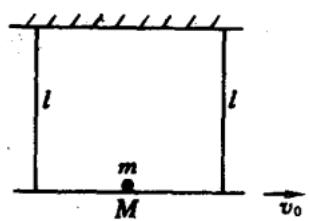
\includegraphics[width=0.3\textwidth]{figures/图_7_35.jpg}
\end{center}

\vfill

\textbf{7-54} 某竖直平面内有一半径为 $R$ 的光滑固定圆环, 斜边长 2R、短边长 $R$ 的匀质直角三角板放在环内, 试求三角板在其平衡位置两侧小角度摆动周期 $T$.

\begin{center}
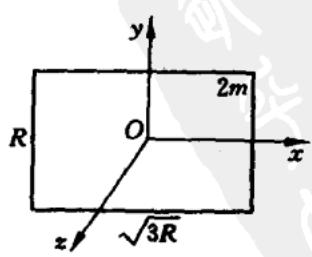
\includegraphics[width=0.3\textwidth]{figures/图_7_39.jpg}
\end{center}

\vfill

\newpage

\textbf{7-55} 半径 $R$ 的匀质圆环截去任何一段圆弧, 以余下的圆弧段的中点为悬挂点, 可形成小角度复摆运动, 试证摆动周期为常量.

\vfill

\textbf{7-56} 在水平光滑细长直角槽中嵌入两个质量相同的小物块 $A$ 和 $B$ , 它们的上表面用长为 $l$ 、质量可忽略的刚性细杆铰接, 铰接处在 $A, B$ 运动时可无摩擦地自由旋转. 开始时, $A, B$ 与细杆都静止, 细杆不平行于任何一条槽, 即图 7-41 中的 $\theta_0$ 为锐角. 然后沿 $x_0$ 方向给 $A$ 施以冲量, 于是 $A, B$ 均会在各自槽中无摩擦地运动.

(1) 试证细杆中点 $C$ 将作圆周运动；

(2) 试证 $A$, $B$ 各自作简谐振动，并且用 $l, \theta_{0}, v_{AO}$ ($A$ 的初速大小) 诸量表述周期 $T$.

\begin{center}
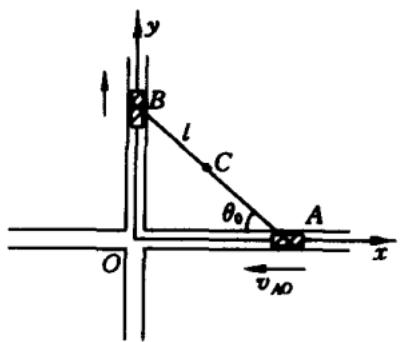
\includegraphics[width=0.3\textwidth]{figures/图7_41.jpg}
\end{center}

\vfill

\newpage

\textbf{7-57} 如图所示, 在水平光滑桌面的中心有一光滑小孔 $O$, 一根劲度系数为 $k$ 的弹性轻绳穿过小孔 $O$, 绳的一端固定于小孔正下方的 $A$ 点, 另一端系一质量为 $m$ 的小球, 弹性绳自由长度等于 $\overline{OA}$ . 现将小球沿桌面拉至 $B$ 处, 设 $\overline{OB}=l$ , 并让小球沿垂直于 OB 的方向以初速度 $v_{0}$ 在桌面上运动. 试求:

(1) 小球绕 $O$ 点转过 $90^{\circ}$ 至 $C$ 点所需时间；

(2) 小球到达 $C$ 点时的速度 $v_{C}$ 及 $C$ 点至 $O$ 点的距离.

\begin{center}
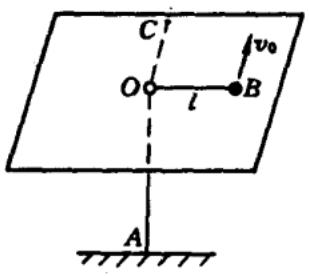
\includegraphics[width=0.2\textwidth]{figures/图7_42.jpg}
\end{center}

\vfill

\textbf{7-58} 如图所示, 质量为 $M$ 、宽为 $d$ 的木块置于光滑水平面上, 与一端固定于竖直墙上的轻弹簧相连, 弹簧的劲度系数为 $k$ , 处于原长. 一质量为 $m$ 的子弹以 $v_0$ 初速度水平射向木块, 在穿入或穿透木块的过程中, 受到木块的摩擦阻力恒为常量 $F$ . 试求木块第一次向右运动过程中速度可能达到的最大值, 以及此时对应的子弹入射速度 $v_0$ .

已知在子弹穿入或穿透木块过程中,木块的质量不因子弹的射入而变化,且有 $kd \geqslant 2F, m/M \geqslant 5/4$ .

\begin{center}
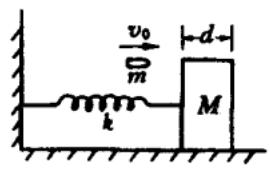
\includegraphics[width=0.2\textwidth]{figures/图7_44.jpg}
\end{center}

\vfill

\newpage

\textbf{7-59} 湖震(第15届国际物理奥林匹克试题2, 1984年, 瑞典斯土纳, 稍有改动.)

在某些湖泊中能经常观察到称之为“湖震”(湖水振动)的奇异现象. 这通常发生在长且较窄的浅水湖中, 全部湖水就像杯中的咖啡在端动时那样地晃动, 可能误以为是水面波的波动.

为构建湖震模型,取一个长 $L$ 的容器,其内盛水高度记为 $h$. 水面初始状态如图所示,其中 $\xi \ll h$ , 水面随即绕容器一半长度处的水平轴振动,且水面始终保持为平面.

(1) 为容器中的水建立较为简单的振动模型, 导出振动周期 $T$ 的算式;

(2) 两组实验数据如下:

<table><tr><td rowspan="2"><eq>L=479 \text{ mm}</eq>:</td><td><eq>h/\text{mm}</eq></td><td>30</td><td>50</td><td>69</td><td>88</td><td>107</td><td>124</td><td>142</td></tr><tr><td><eq>T/\text{s}</eq></td><td>1.78</td><td>1.40</td><td>1.18</td><td>1.08</td><td>1.00</td><td>0.91</td><td>0.82</td></tr><tr><td rowspan="2"><eq>L=143 \text{ mm}</eq>:</td><td><eq>h/\text{mm}</eq></td><td>31</td><td>38</td><td>58</td><td>67</td><td>124</td><td></td><td></td></tr><tr><td><eq>T/\text{s}</eq></td><td>0.52</td><td>0.48</td><td>0.43</td><td>0.35</td><td>0.28</td><td></td><td></td></tr></table>

据(1)问解答算出相应的周期 $T$, 估计理论误差.

\begin{center}
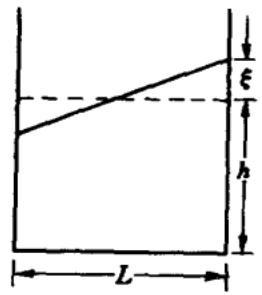
\includegraphics[width=0.2\textwidth]{figures/图7_46.jpg}
\end{center}

\vfill

\textbf{7-60} 如图所示, 水平桌面上有一质量 $M$、半径 $R$ 的细管状匀质圆环, 环内有三根轻质细管状辐条, 辐条连通环心, 环心 $O$ 套在一根固定的竖直细轴上, 环可绕此轴在水平桌面上转动. $O$ 处连接一根自由长度为 $R$、劲度系数为 $k$ 的弹性轻绳, 轻绳通过一根辐条内壁到达圆环细管, 拉长到图示的 $\theta_{0}<\frac{2}{3}\pi$ 处, 连接一个质量为 $m$ 的小球. 开始时圆环和小球均处于静止状态, 而后小球在圆环细管内运动, 圆环绕 $O$ 轴转动. 假设系统处处无摩擦, 试求:

(1) 系统运动周期 $T$;

(2) 小球刚开始运动时转轴提供的支持力大小 $N_{1}$ 和小球到达辐条端位处时转轴提供的支持力大小 $N_{2}$ .

\begin{center}
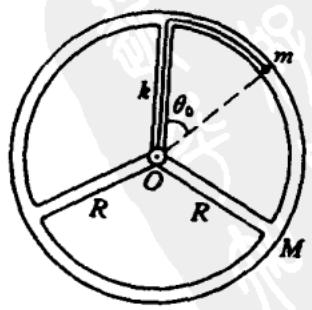
\includegraphics[width=0.2\textwidth]{figures/图7_48.jpg}
\end{center}

\vfill

\newpage

\textbf{7-61} 直线 $MN$ 上的 $O$ 点两侧有两个电量同为 $Q > 0$ 的固定点电荷, 各自与 $O$ 点的距离同为 $a$ . 一根固定的光滑绝缘细管过 $O$ 点, 且与直线 $MN$ 的夹角为 $\phi \left(\frac{\pi}{2} \geqslant \phi \geqslant 0\right)$ . 如图所示, 质量 $m$ 、电量 $q > 0$ 的带电质点可在管内 $O$ 点静止地处于平衡状态.

(1) 判断带电质点所处平衡位置的稳定性；

(2) 如果是稳定平衡位置, 而且当带电质点稍稍偏离该平衡位置时沿细管方向所受力为线性回复力, 则求其小振动周期 $T$.

\begin{center}
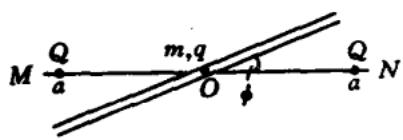
\includegraphics[width=0.3\textwidth]{figures/图7_49.jpg}
\end{center}

\vfill

\textbf{7-62} 导出摆长 $l$、幅角 $\theta_{0}$ 单摆的摆动周期 $T$ 的严格解，并给出一级和二级近似解.


\vfill

\newpage

\textbf{7-63} 如图所示, 半径 $R$ 的圆环绕铅垂的直径轴以角速度 $\omega$ 匀速旋转. 匀质细杆长 $L = \sqrt{2} R$ , 两端约束在环上可作无摩擦的滑动, 细杆的位置用 OC 与铅垂轴的夹角 $\theta$ 表示, $O$ 是环心, $C$ 是杆的中心. 试求细杆在环内的平衡位置, 并讨论平衡的稳定性.

\begin{center}
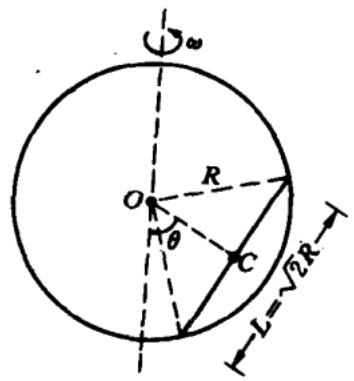
\includegraphics[width=0.2\textwidth]{figures/图_7_51.jpg}
\end{center}

\vfill

\textbf{7-64} 一种耦合振子的具体结构和相关参量如图所示, 其中 $x_{1}, x_{2}$ 分别是左、右振子沿 $x$ 轴偏离各自平衡点的位移量. 已知 $x_{1} = 0; x_{2} = 0$ 时三根轻弹簧均无形变, 水平地面光滑, 试求 $x_{1} - t, x_{2} - t$ 的通解.

\begin{center}
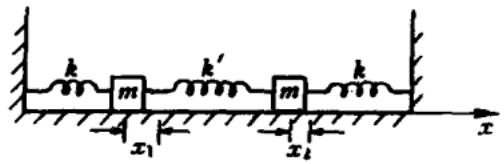
\includegraphics[width=0.3\textwidth]{figures/图7_53.jpg}
\end{center}

\vfill

\newpage

\textbf{7-65} 质量为 $m$ 的小物块悬挂于劲度系数为 $k$ 的弹簧下端, 平衡于 $O$ 点. 如图所示, 从 $t = 0$ 开始, 弹簧上端 $O'$ 以 $x' = a \sin \omega t$ 的方式做上、下振动 (以向下为正). 已知空气阻力系数为 $\gamma$ , 设置以 $O$ 为原点、竖直向下的 $x$ 轴, 试求系统达到稳定运动状态后, 小物块的位置 $x$ 随时间 $t$ 的变化关系.

\begin{center}
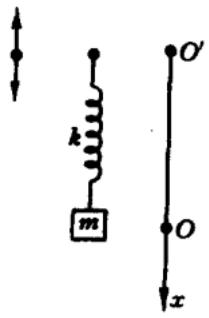
\includegraphics[width=0.15\textwidth]{figures/图_7_54.jpg}
\end{center}

\vfill

\textbf{7-66} 一振子在驱动力 $F = F_{0} \cos \omega t$ 作用下形成受迫振动. 已知振子质量 $m = 0.2 \mathrm{~kg}$ , 弹簧劲度系数 $k = 80 \mathrm{~N} / \mathrm{m}$ , 阻力系数 $\gamma = 4 \mathrm{~N} \cdot \mathrm{s} / \mathrm{m}, F_{0} = 2 \mathrm{~N}, \omega = 30 / \mathrm{s}$ , 达稳态后试求:

(1) 振子系统在一个周期内反抗阻力而耗散的能量；

(2) 驱动力输入系统的平均功率.

\vfill

\newpage

\textbf{7-67} 运动学方程为 $\xi_{i} = A\cos \left(\omega t - \frac{2\pi}{\lambda} x\right)$ 的入射波在弦线上沿 $x$ 方向传播，弦线的质量线密度为 $\lambda_{m}$ ，弦中张力为 $T$ ，在 $x = 0$ 处有一质量为 $m$ 的质点固定于弦上，如图所示.将 $x = 0$ 处的反射波和透射波分别记为
\[
\xi_ {\mathrm{r}} = B \cos \left(\omega t + \frac {2 \pi}{\lambda} x + \phi_ {\mathrm{r}}\right), \quad \xi_ {\mathrm{t}} = C \cos \left(\omega t - \frac {2 \pi}{\lambda} x + \phi_ {\mathrm{t}}\right),
\]
试求 $\phi_{r},\phi_{t}$ 和 $B$,$C$.（答案用 $A$, $\omega,\lambda_{m},T,m$ 表述.）

\begin{center}
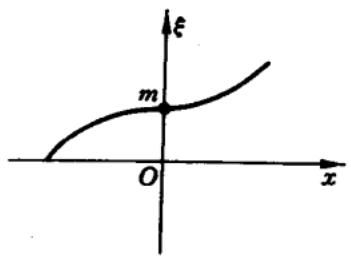
\includegraphics[width=0.3\textwidth]{figures/图7_55.jpg}
\end{center}

\vfill
